\documentclass{extbook}[14pt]
\usepackage{multicol, enumerate, enumitem, hyperref, color, soul, setspace, parskip, fancyhdr, amssymb, amsthm, amsmath, bbm, latexsym, units, mathtools}
\everymath{\displaystyle}
\usepackage[headsep=0.5cm,headheight=0cm, left=1 in,right= 1 in,top= 1 in,bottom= 1 in]{geometry}
\usepackage{dashrule}  % Package to use the command below to create lines between items
\newcommand{\litem}[1]{\item #1

\rule{\textwidth}{0.4pt}}
\pagestyle{fancy}
\lhead{}
\chead{Answer Key for Progress Quiz 4 Version B}
\rhead{}
\lfoot{6286-1986}
\cfoot{}
\rfoot{Fall 2020}
\begin{document}
\textbf{This key should allow you to understand why you choose the option you did (beyond just getting a question right or wrong). \href{https://xronos.clas.ufl.edu/mac1105spring2020/courseDescriptionAndMisc/Exams/LearningFromResults}{More instructions on how to use this key can be found here}.}

\textbf{If you have a suggestion to make the keys better, \href{https://forms.gle/CZkbZmPbC9XALEE88}{please fill out the short survey here}.}

\textit{Note: This key is auto-generated and may contain issues and/or errors. The keys are reviewed after each exam to ensure grading is done accurately. If there are issues (like duplicate options), they are noted in the offline gradebook. The keys are a work-in-progress to give students as many resources to improve as possible.}

\rule{\textwidth}{0.4pt}

\begin{enumerate}\litem{
Describe the end behavior of the polynomial below.
\[ f(x) = 9(x + 6)^{5}(x - 6)^{10}(x + 3)^{3}(x - 3)^{5} \]
The solution is the graph below, which is option D.
\begin{center}
    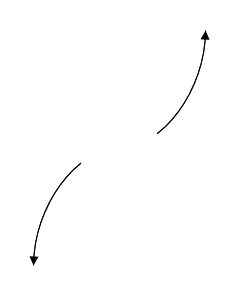
\includegraphics[width=0.3\textwidth]{../Figures/polyEndBehaviorCopyDB.png}
\end{center}\begin{enumerate}[label=\Alph*.]
\begin{multicols}{2}
\item 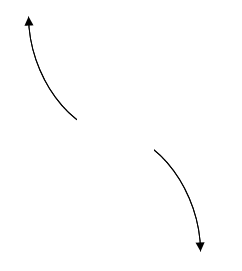
\includegraphics[width = 0.3\textwidth]{../Figures/polyEndBehaviorCopyAB.png}
\item 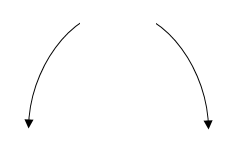
\includegraphics[width = 0.3\textwidth]{../Figures/polyEndBehaviorCopyBB.png}
\item 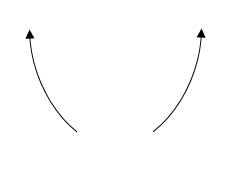
\includegraphics[width = 0.3\textwidth]{../Figures/polyEndBehaviorCopyCB.png}
\item 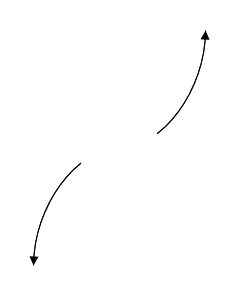
\includegraphics[width = 0.3\textwidth]{../Figures/polyEndBehaviorCopyDB.png}
\end{multicols}\item None of the above.\end{enumerate}
\textbf{General Comment:} Remember that end behavior is determined by the leading coefficient AND whether the \textbf{sum} of the multiplicities is positive or negative.
}
\litem{
Construct the lowest-degree polynomial given the zeros below. Then, choose the intervals that contain the coefficients of the polynomial in the form $ax^3+bx^2+cx+d$.
\[ 7, 6, \text{ and } \frac{-7}{4} \]
The solution is \( 4x^{3} -45 x^{2} +77 x + 294 \), which is option C.\begin{enumerate}[label=\Alph*.]
\item \( a \in [-1, 5], b \in [-51, -40], c \in [74, 78], \text{ and } d \in [-295, -287] \)

$4x^{3} -45 x^{2} +77 x -294$, which corresponds to multiplying everything correctly except the constant term.
\item \( a \in [-1, 5], b \in [43, 49], c \in [74, 78], \text{ and } d \in [-295, -287] \)

$4x^{3} +45 x^{2} +77 x -294$, which corresponds to multiplying out $(x + 7)(x + 6)(4x -7)$.
\item \( a \in [-1, 5], b \in [-51, -40], c \in [74, 78], \text{ and } d \in [287, 297] \)

* $4x^{3} -45 x^{2} +77 x + 294$, which is the correct option.
\item \( a \in [-1, 5], b \in [58, 62], c \in [256, 261], \text{ and } d \in [287, 297] \)

$4x^{3} +59 x^{2} +259 x + 294$, which corresponds to multiplying out $(x + 1)(x + 1)(4x -4)$.
\item \( a \in [-1, 5], b \in [11, 13], c \in [-164, -157], \text{ and } d \in [-295, -287] \)

$4x^{3} +11 x^{2} -161 x -294$, which corresponds to multiplying out $(x + 1)(x -1)(4x -4)$.
\end{enumerate}

\textbf{General Comment:} To construct the lowest-degree polynomial, you want to multiply out $(x -7)(x -6)(4x + 7)$
}
\litem{
Construct the lowest-degree polynomial given the zeros below. Then, choose the intervals that contain the coefficients of the polynomial in the form $x^3+bx^2+cx+d$.
\[ -4 + 2 i \text{ and } -3 \]
The solution is \( x^{3} +11 x^{2} +44 x + 60 \), which is option B.\begin{enumerate}[label=\Alph*.]
\item \( b \in [-1, 7], c \in [-1, 4], \text{ and } d \in [-13, -3] \)

$x^{3} + x^{2} +x -6$, which corresponds to multiplying out $(x -2)(x + 3)$.
\item \( b \in [10, 18], c \in [41, 45], \text{ and } d \in [55, 73] \)

* $x^{3} +11 x^{2} +44 x + 60$, which is the correct option.
\item \( b \in [-11, -4], c \in [41, 45], \text{ and } d \in [-60, -58] \)

$x^{3} -11 x^{2} +44 x -60$, which corresponds to multiplying out $(x-(-4 + 2 i))(x-(-4 - 2 i))(x -3)$.
\item \( b \in [-1, 7], c \in [7, 13], \text{ and } d \in [8, 17] \)

$x^{3} + x^{2} +7 x + 12$, which corresponds to multiplying out $(x + 4)(x + 3)$.
\item \( \text{None of the above.} \)

This corresponds to making an unanticipated error or not understanding how to use nonreal complex numbers to create the lowest-degree polynomial. If you chose this and are not sure what you did wrong, please contact the coordinator for help.
\end{enumerate}

\textbf{General Comment:} Remember that the conjugate of $a+bi$ is $a-bi$. Since these zeros always come in pairs, we need to multiply out $(x-(-4 + 2 i))(x-(-4 - 2 i))(x-(-3))$.
}
\litem{
Describe the end behavior of the polynomial below.
\[ f(x) = -8(x - 4)^{5}(x + 4)^{8}(x + 3)^{4}(x - 3)^{6} \]
The solution is the graph below, which is option A.
\begin{center}
    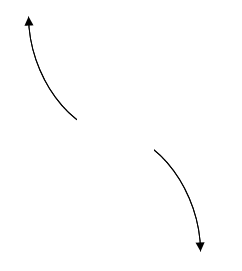
\includegraphics[width=0.3\textwidth]{../Figures/polyEndBehaviorAB.png}
\end{center}\begin{enumerate}[label=\Alph*.]
\begin{multicols}{2}
\item 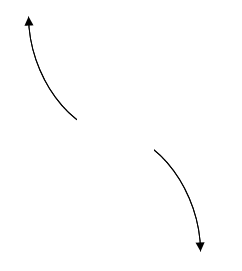
\includegraphics[width = 0.3\textwidth]{../Figures/polyEndBehaviorAB.png}
\item 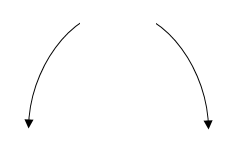
\includegraphics[width = 0.3\textwidth]{../Figures/polyEndBehaviorBB.png}
\item 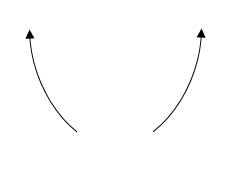
\includegraphics[width = 0.3\textwidth]{../Figures/polyEndBehaviorCB.png}
\item 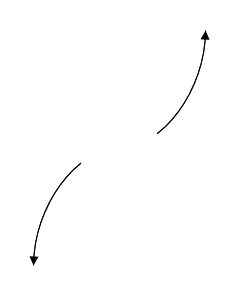
\includegraphics[width = 0.3\textwidth]{../Figures/polyEndBehaviorDB.png}
\end{multicols}\item None of the above.\end{enumerate}
\textbf{General Comment:} Remember that end behavior is determined by the leading coefficient AND whether the \textbf{sum} of the multiplicities is positive or negative.
}
\litem{
Which of the following equations \textit{could} be of the graph presented below?

\begin{center}
    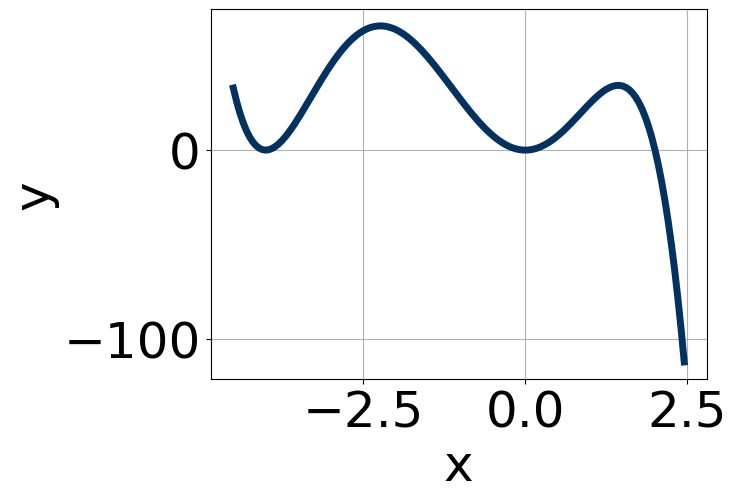
\includegraphics[width=0.5\textwidth]{../Figures/polyGraphToFunctionCopyB.png}
\end{center}



The solution is \( -8(x - 2)^{10} (x - 3)^{4} (x + 2)^{9} \), which is option C.\begin{enumerate}[label=\Alph*.]
\item \( 13(x - 2)^{10} (x - 3)^{4} (x + 2)^{4} \)

The factor $(x + 2)$ should have an odd power and the leading coefficient should be the opposite sign.
\item \( 2(x - 2)^{8} (x - 3)^{10} (x + 2)^{7} \)

This corresponds to the leading coefficient being the opposite value than it should be.
\item \( -8(x - 2)^{10} (x - 3)^{4} (x + 2)^{9} \)

* This is the correct option.
\item \( -3(x - 2)^{4} (x - 3)^{5} (x + 2)^{9} \)

The factor $(x - 3)$ should have an even power.
\item \( -16(x - 2)^{6} (x - 3)^{7} (x + 2)^{10} \)

The factor $(x - 3)$ should have an even power and the factor $(x + 2)$ should have an odd power.
\end{enumerate}

\textbf{General Comment:} General Comments: Draw the x-axis to determine which zeros are touching (and so have even multiplicity) or cross (and have odd multiplicity).
}
\litem{
Which of the following equations \textit{could} be of the graph presented below?

\begin{center}
    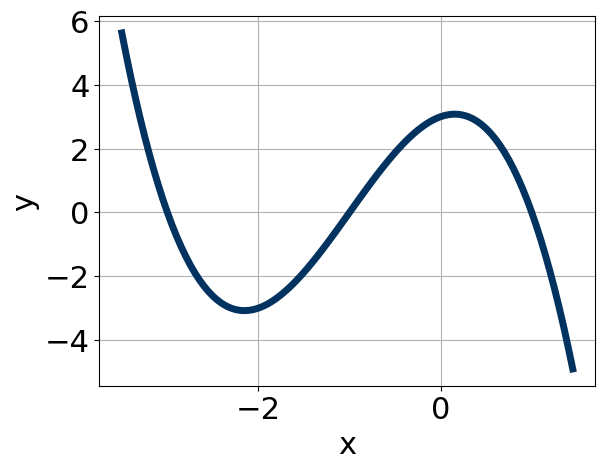
\includegraphics[width=0.5\textwidth]{../Figures/polyGraphToFunctionB.png}
\end{center}



The solution is \( 13x^{8} (x - 2)^{5} (x + 1)^{7} \), which is option E.\begin{enumerate}[label=\Alph*.]
\item \( 13x^{10} (x - 2)^{4} (x + 1)^{11} \)

The factor $(x - 2)$ should have an odd power.
\item \( -8x^{6} (x - 2)^{5} (x + 1)^{4} \)

The factor $(x + 1)$ should have an odd power and the leading coefficient should be the opposite sign.
\item \( -16x^{8} (x - 2)^{5} (x + 1)^{5} \)

This corresponds to the leading coefficient being the opposite value than it should be.
\item \( 3x^{11} (x - 2)^{6} (x + 1)^{9} \)

The factor $0$ should have an even power and the factor $2$ should have an odd power.
\item \( 13x^{8} (x - 2)^{5} (x + 1)^{7} \)

* This is the correct option.
\end{enumerate}

\textbf{General Comment:} General Comments: Draw the x-axis to determine which zeros are touching (and so have even multiplicity) or cross (and have odd multiplicity).
}
\litem{
Construct the lowest-degree polynomial given the zeros below. Then, choose the intervals that contain the coefficients of the polynomial in the form $ax^3+bx^2+cx+d$.
\[ \frac{-4}{5}, \frac{-2}{3}, \text{ and } 3 \]
The solution is \( 15x^{3} -23 x^{2} -58 x -24 \), which is option A.\begin{enumerate}[label=\Alph*.]
\item \( a \in [10, 22], b \in [-24, -20], c \in [-64, -57], \text{ and } d \in [-24, -18] \)

* $15x^{3} -23 x^{2} -58 x -24$, which is the correct option.
\item \( a \in [10, 22], b \in [-51, -42], c \in [-8, 5], \text{ and } d \in [22, 29] \)

$15x^{3} -47 x^{2} -2 x + 24$, which corresponds to multiplying out $(5x + 5)(3x -3)(x -1)$.
\item \( a \in [10, 22], b \in [-70, -60], c \in [74, 80], \text{ and } d \in [-24, -18] \)

$15x^{3} -67 x^{2} +74 x -24$, which corresponds to multiplying out $(5x + 5)(3x + 3)(x -1)$.
\item \( a \in [10, 22], b \in [-24, -20], c \in [-64, -57], \text{ and } d \in [22, 29] \)

$15x^{3} -23 x^{2} -58 x + 24$, which corresponds to multiplying everything correctly except the constant term.
\item \( a \in [10, 22], b \in [18, 27], c \in [-64, -57], \text{ and } d \in [22, 29] \)

$15x^{3} +23 x^{2} -58 x + 24$, which corresponds to multiplying out $(5x -4)(3x -2)(x + 3)$.
\end{enumerate}

\textbf{General Comment:} To construct the lowest-degree polynomial, you want to multiply out $(5x + 4)(3x + 2)(x -3)$
}
\litem{
Describe the zero behavior of the zero $x = 9$ of the polynomial below.
\[ f(x) = 7(x - 9)^{6}(x + 9)^{7}(x - 6)^{7}(x + 6)^{11} \]
The solution is the graph below, which is option C.
\begin{center}
    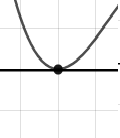
\includegraphics[width=0.3\textwidth]{../Figures/polyZeroBehaviorCopyCB.png}
\end{center}\begin{enumerate}[label=\Alph*.]
\begin{multicols}{2}
\item 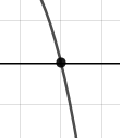
\includegraphics[width = 0.3\textwidth]{../Figures/polyZeroBehaviorCopyAB.png}
\item 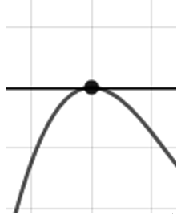
\includegraphics[width = 0.3\textwidth]{../Figures/polyZeroBehaviorCopyBB.png}
\item 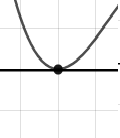
\includegraphics[width = 0.3\textwidth]{../Figures/polyZeroBehaviorCopyCB.png}
\item 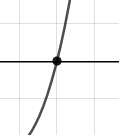
\includegraphics[width = 0.3\textwidth]{../Figures/polyZeroBehaviorCopyDB.png}
\end{multicols}\item None of the above.\end{enumerate}
\textbf{General Comment:} You will need to sketch the entire graph, then zoom in on the zero the question asks about.
}
\litem{
Construct the lowest-degree polynomial given the zeros below. Then, choose the intervals that contain the coefficients of the polynomial in the form $x^3+bx^2+cx+d$.
\[ -4 - 3 i \text{ and } -2 \]
The solution is \( x^{3} +10 x^{2} +41 x + 50 \), which is option C.\begin{enumerate}[label=\Alph*.]
\item \( b \in [0, 7], c \in [3.09, 5.81], \text{ and } d \in [5.4, 7.3] \)

$x^{3} + x^{2} +5 x + 6$, which corresponds to multiplying out $(x + 3)(x + 2)$.
\item \( b \in [-10, -3], c \in [40.53, 42.29], \text{ and } d \in [-52, -49.7] \)

$x^{3} -10 x^{2} +41 x -50$, which corresponds to multiplying out $(x-(-4 - 3 i))(x-(-4 + 3 i))(x -2)$.
\item \( b \in [9, 16], c \in [40.53, 42.29], \text{ and } d \in [49, 50.4] \)

* $x^{3} +10 x^{2} +41 x + 50$, which is the correct option.
\item \( b \in [0, 7], c \in [5.46, 7.06], \text{ and } d \in [7, 11.7] \)

$x^{3} + x^{2} +6 x + 8$, which corresponds to multiplying out $(x + 4)(x + 2)$.
\item \( \text{None of the above.} \)

This corresponds to making an unanticipated error or not understanding how to use nonreal complex numbers to create the lowest-degree polynomial. If you chose this and are not sure what you did wrong, please contact the coordinator for help.
\end{enumerate}

\textbf{General Comment:} Remember that the conjugate of $a+bi$ is $a-bi$. Since these zeros always come in pairs, we need to multiply out $(x-(-4 - 3 i))(x-(-4 + 3 i))(x-(-2))$.
}
\litem{
Describe the zero behavior of the zero $x = 5$ of the polynomial below.
\[ f(x) = 2(x + 5)^{3}(x - 5)^{8}(x + 7)^{9}(x - 7)^{10} \]
The solution is the graph below, which is option C.
\begin{center}
    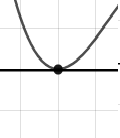
\includegraphics[width=0.3\textwidth]{../Figures/polyZeroBehaviorCB.png}
\end{center}\begin{enumerate}[label=\Alph*.]
\begin{multicols}{2}
\item 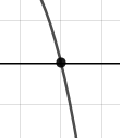
\includegraphics[width = 0.3\textwidth]{../Figures/polyZeroBehaviorAB.png}
\item 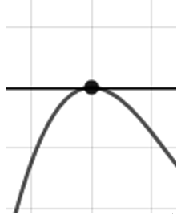
\includegraphics[width = 0.3\textwidth]{../Figures/polyZeroBehaviorBB.png}
\item 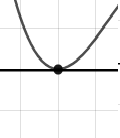
\includegraphics[width = 0.3\textwidth]{../Figures/polyZeroBehaviorCB.png}
\item 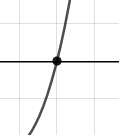
\includegraphics[width = 0.3\textwidth]{../Figures/polyZeroBehaviorDB.png}
\end{multicols}\item None of the above.\end{enumerate}
\textbf{General Comment:} You will need to sketch the entire graph, then zoom in on the zero the question asks about.
}
\end{enumerate}

\end{document}